%
%  Thesis Vorlage für die Hochschule Heilbronn
%
%  Created by Prof. Dr. Detlef Stern on 2010-08-14.
%  Updated by Valentin Weber on 2020-10-05.
%  Copyright (c) 2020 . All rights reserved.
%
\documentclass[12pt,toc=bib,toc=listof]{scrreprt}
\usepackage[ngerman]{babel} 
\usepackage[utf8]{inputenc}
\usepackage[T1]{fontenc}
\usepackage{lmodern}
\usepackage{setspace}
\usepackage{geometry}

\usepackage{hyperref}
\hypersetup{
  ,colorlinks=true
  ,linkcolor=blue
  ,citecolor=blue
  ,filecolor=blue
  ,urlcolor=blue
  }

% Fachbezogene Werte (müssen aktualisiert werden)
\newcommand{\hhnsubject}{COMPUTER AND ROBOTVISION}
\newcommand{\hhnsubjectnum}{PRÜFUNGSNUMMER: 135031}
\newcommand{\hhnlecturer}{PROF. DR. DIETER MAIER}

% Vom Studierenden zu aendernde Werte
\newcommand{\reprttopic}{BRIEFMARKENERKENNUNG}
\newcommand{\reprtstudentname}{GEORG JAHN, MARTIN HAAG}
\newcommand{\reprtstudentid}{195XXX, 194980}
\urldef{\reprtstudentmail}\url{gjahn@stud.hs-heilbronn.de ,mahaag@stud.hs-heilbronn.de}

\usepackage{ifpdf}
\ifpdf
\usepackage[pdftex]{graphicx}
\else
\usepackage{graphicx}
\fi

\usepackage[headsepline]{scrlayer-scrpage}
\pagestyle{scrheadings}
\clearscrheadfoot
\ihead{\hhnsubject: \reprttopic}
\ohead{\pagemark}
\renewcommand*{\chapterpagestyle}{scrheadings}
\renewcommand*{\chapterheadstartvskip}{}

%meine adds
\usepackage[belowskip=-15pt,aboveskip=0pt]{caption}
\renewcommand*{\figurename}{Abb.}

% Deckblatt Definitionen (begin)
\titlehead{\flushright
\includegraphics{./bilder/hhn.png}}
\subject{{\hhnsubject{} (\hhnsubjectnum{})}}
\title{\reprttopic}
\author{\reprtstudentname\footnote{\reprtstudentid, \reprtstudentmail}}
%% Datum nie auf einen festen Wert setzen
\publishers{Eingereicht bei \hhnlecturer}
% Deckblatt Definitionen (end)

\begin{document}
\renewcommand*{\figurename}{Abb.}
\pagenumbering{Roman} 
\selectlanguage{ngerman}
\maketitle
\newgeometry{left=30mm, top=25mm, right=15mm, bottom=25mm}

\tableofcontents

\addchap{List of Abbreviations} % (fold)
\label{sec:listofabbrv}

\addchap{Abkürzungsverzeichnis} % (fold)
\label{sec:abkuerzungsverzeichnis}

\begin{description}
  \item[ABK:] ABKÜRZUNG 
\end{description}

% chapter abkuerzungsverzeichnis (end)

\onehalfspacing

\addchap{Management Summary} % (fold)
\label{cha:management_summary}
\ldots

% chapter management_summary (end)
\newpage
\pagenumbering{arabic}

% report (begin)
\chapter{Einleitung} % (fold)
\label{sec:einleitung}

\section{Motivation} % (fold)
\label{sec:motivation}

Bildverarbeitung ist kein neues Feld der Forschung mehr und auch neuronale Netzwerke sind bereits seit vielen Jahren Subjekt von ständiger Weiterentwicklung. Da diese beiden Fachgebiete durchaus gut miteinander harmonieren haben wir uns entschieden, in unserem Projekt eine Aufgabe die beides benötigt zu bearbeiten. Im Rahmen useres CRV Projektes haben wir deshalb die Unterscheidung von Briefmarken in gestempelte und ungestempelte automatisiert, durchgeführt. Wenn auch unsere Arbeit sehr unwahrscheinlich kommerzielle Anwendung findet, ist es doch geeignet um an einem Tag der offenen Tür oder einem "studieren probieren" Event demonstriert zu werden.

% section motivation (end)

\section{Ziel der Arbeit} % (fold)
\label{sec:ziel_der_arbeit}
Das Ziel der Arbeit war es, mit Hilfe eines Teils "klassischer" Bildverarbeitung und eins neuronalen Netzwerkes Bilder von gestempelten von Bildern mit ungestempelten Briefmarken zu unterscheiden.
Ursprünglich war der Plan mit Bildern von ganzen Briefen zu arbeiten. Der Vorteil bei diesem Ansatz wäre, dass die Überlappung des Stempels über Briefmarke und Brief es wohl für das Netzwerk einfacher gemacht hätte die Klassen gestempelt/nicht gestempelt zu unterscheiden. Auf Grund von Datenschutzgesetzten waren wir jedoch nicht in der Lage, einen ausreichend großen Datensatz zusammen zu tragen. Deshalb haben wir uns entschieden, eine alte selbst gesammelte Briefmarkensammlung abzufotografieren und somit zu digitalisieren.


Dieser selbst generierte Datensatz ist zwar auch nicht groß genug um ein ernsthaftes Training mit einem NN durchzuführen, reicht aber für einen "Proof of concept"

% section ziel_der_arbeit (end)

\section{Vorgehensweise} % (fold)
\label{sec:vorgehensweise}

Unser Vorgehen teilt sich in zwei Teilschritte auf:
\begin{itemize}
\item "klassische" Bildverarbeitung:\\ 
Dabei werden die Bilder so vorverarbeitet, dass sie als Input für das NN dienen können. Das wird mit Hilfe von helligkeitsbasierte Binarisierung und einigen morphologischen Filtern erreicht. Außerdem kommen noch Schritte zum drehen des Bildes zum Einsatz. Das Endergebniss dieser Bildverarbeitungsschritte ist ein rechteckiger Bildausschnitt, der nur die Briefmarke enthält. 

\item Klassifizierung mit einem NN:\\
In diesem Bereich der Arbeit wird der vorverarbeitete Datensatz für das Training und die Evaluierung des NN aufbereitet. Außerdem wird das NN selbst hier erstellt. Da wir die Technik des Transferlearning genutzt haben, wurde hier nur ein vortrainiertes Model herausgesucht und das Outputlayer ausgetauscht.

\end{itemize}

% section vorgehensweise (end)
% chapter einleitung (end)

\chapter{Klassische Bildverarbeitung} % (fold)
\label{sec:klass_bv}

\section{Übersicht}
\label{sec_bv:übersicht}
Das folgende Schaubild zeigt, welche Schritte vorgenommen werden und in welcher Reihenfolge. Dafür wurde ein Beispiel gewählt, bei dem keine Komplikationen auftreten.
\begin{figure}[h]
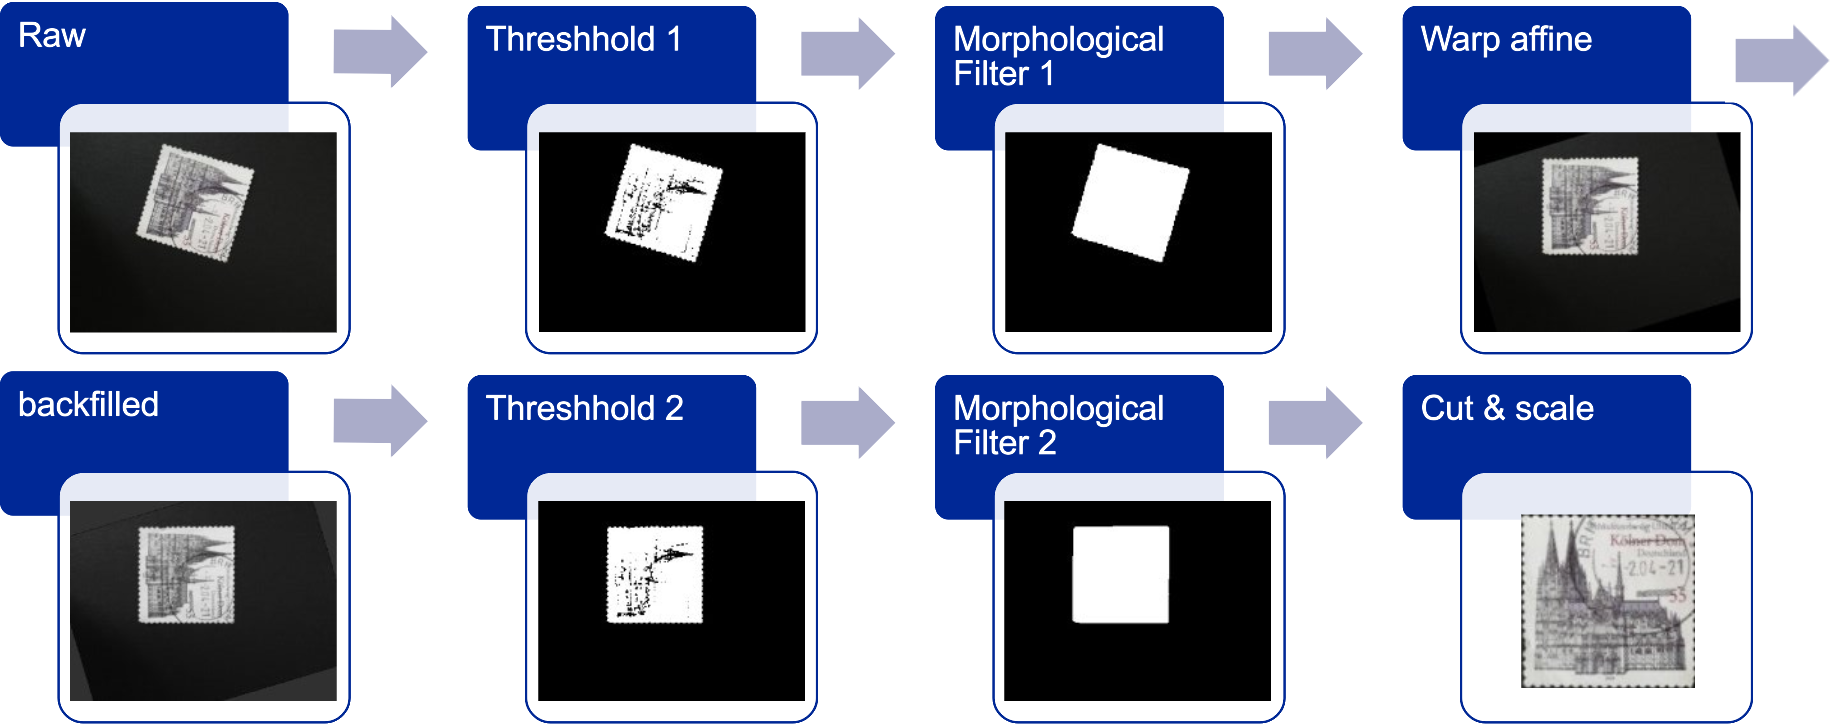
\includegraphics[width=\textwidth]{./bilder/bv_overview.png}
\caption{Übersicht über die Schritte der Bildvorverarbeitung}
\label{fig:bv_overview}
\end{figure}


\begin{figure}[t]

\begin{minipage}[t]{.6\linewidth}
Die beiden Bilder auf der rechten Seite sind Eingang und Ausgang des ersten Schrittes (Raw -> Threshold1). Das Raw Bild ist dabei ein RGB Bild, auf dem die Briefmarke in zufälliger Orientierung zu sehen ist. Der Hindergrund ist matt und schwarz-grau. Der Übergang zu Threshold1 wird mit einer Otsu Binarisierung bewerkstelligt. Es wird also in ein Graustufenbild übergegangen. Je nach Motiv der Briefmarke sind im Binärbild jedoch noch viele schwarze Stellen auf der Briefmarke. Dadurch resultiert die Marke nicht in einer einzelnen großen Kontur, sondern in vielen kleinen. Da wir jedoch erstmal das Bild gerade drehen wollen, bräuchten wir dafür eine einzige große, möglichst rechteckige, Kontur.
\end{minipage}
\hspace{0.02\linewidth}
\begin{minipage}[t]{.2\linewidth}
  \strut\vspace*{-\baselineskip}\newline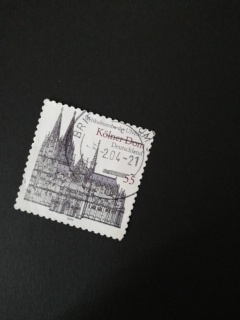
\includegraphics[width=\linewidth]{./bilder/start_dom}
  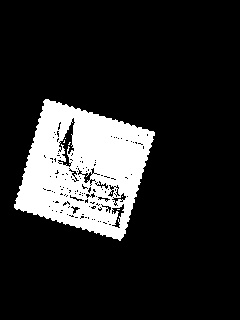
\includegraphics[width=\linewidth]{./bilder/bin1_dom}
  \caption{Übergang zu Threshold1}
  \label{fig:bv_th1}
\end{minipage}
\end{figure}
%%% ggf. weitere Abschnitte

\begin{figure}[h]
\begin{minipage}[t]{.6\linewidth}

Die Abbilung \ref{fig:bv_morph1} zeigt das Ergebnis des zweiten Schrittes des "klassischen" Teiles. Hier sind keine dunklen Stellen mehr auf der Fläche der Briefmarke. Das wurde durch die Verwendung eines morphologischen Filters zur Erweiterung und Schließung von Konturen erreicht. Es wurde dafür eine Quadratische Matrix mit Größe 11x11 verwendet. Bei einer Auflösung von 320x240 ist das ganz stattlich.
\end{minipage}
\begin{minipage}[t]{.2\linewidth}
\strut\vspace*{-\baselineskip}
\newline
  
\includegraphics[width=\linewidth]{./bilder/bin1morph}
  \caption{Übergang zu morph. Filter1}
  \label{fig:bv_morph1}
\end{minipage}
\end{figure}


\chapter{Fazit} % (fold)
\label{sec:fazit}

\ldots

% chapter fazit (end)

\appendix
\begin{thebibliography}{99}
\raggedright
%%% Printquellen zuerst
%%% Beispiel
\bibitem{Th11} Manuel René Theisen:
 \emph{Wissenschaftliches Arbeiten: Technik -- Methodik -- Form};
 15.~Auflage; Vahlen; München 2011;
 ISBN 978-3-8006-3830-7

%%% Internetquellen: Beispiel
\bibitem{hhneb} \emph{Hochschule Heilbronn};
 \url{http://www.hs-heilbronn.de/};
 abgerufen am 14.08.2010
\end{thebibliography}
\end{document}
